%%%%%%%%%%%%%%%%%%%%%%%%%%%%%%%%%%%%%%%%%
%
% Optics and Radar -based observations
% Assignment 3
%
%%%%%%%%%%%%%%%%%%%%%%%%%%%%%%%%%%%%%%%%%

%----------------------------------------------------------------------------------------
%	DOCUMENT CONFIGURATIONS
%----------------------------------------------------------------------------------------

\documentclass{article}

\title{\textbf {Optics and Radar Based Observations} \\ Assignment 3\\ Optimization of phased array antenna radiation pattern and array configuration} % Title
\def\authorivan{Ivan \v Sinkarenko}
\def\authoranu{Anuraj Rajendraprakash}
\author{\authorivan\\\authoranu}

\usepackage{graphicx}
\usepackage{fullpage}
\usepackage{url}

% load package with ``framed'' and ``numbered'' option.
\usepackage[framed,numbered,autolinebreaks,useliterate]{mcode}

\begin{document}

\maketitle % Insert the title, author and date

\centerline{Referee: Dr. Anita Enmark}

\setlength\parindent{0pt} % Removes all indentation from paragraphs

\renewcommand{\labelenumi}{\alph{enumi}.} % Make numbering in the enumerate environment by letter rather than number (e.g. section 6)
\clearpage

\tableofcontents

\listoffigures

\clearpage

%----------------------------------------------------------------------------------------
%	SECTION 1. Introduction
%----------------------------------------------------------------------------------------

\section{Introduction}
A phased array is an array of antennas in which the relative phases of the respective signals feeding the antennas are varied in such a way that the effective radiation pattern of the array is reinforced in a desired direction and suppressed in undesired directions. \cite{Wiki:2012pa}\\

\begin{figure}[h!bt]
\centering
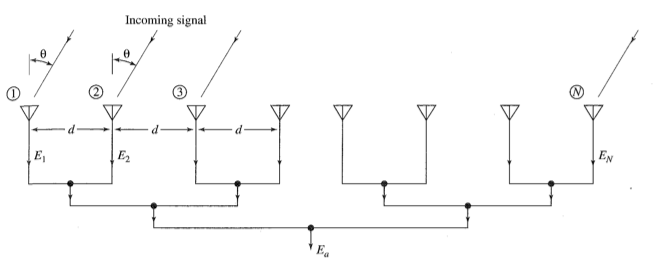
\includegraphics[width=0.7\textwidth]{Figures/phased_array.png}
\caption{N-element receiving, parallel-feed, linear array, with equal lengths of transmission lines between each antenna element and the antenna output (at the bottom on the figure).}
\label{fig:phased_array}
\end{figure}


Consider, as in Figure \ref{fig:phased_array}, a receiving linear array made up of $N$ elements equally spaced a distance $d$ apart. The elements are assumed to be isotropic radiators in that they have uniform response for signals from all directions. Although isotropic radiators are not realizable in practice, they are convenient concept in array theory. The outputs received from all $N$ elements are summed via lines of equal length to produce a sum output voltage $E_a$. Element 1 will be taken as the reference with zero phase. From simple geometry, the difference in path length between adjacent elements for signals arriving at an angle $\theta$ with respect to the normal to the antenna, is $d\,sin\theta$. This gives a phase difference between adjacent elements of $\phi=2\pi(d/\lambda)\,sin\theta$, where $\lambda$ = wavelength of the received signal. It is assumed that there is no further amplitude or phase weighting of the received signals. For convenience, we take the amplitude of the received signal at each element to be unity. The sum of all the voltages from the individual elements, when the phase difference between adjacent elements is $\phi$ can be written
\begin{equation}
\label{eq:first}
E_a=sin\,\omega t+sin(\omega t + \phi)+sin(\omega t + 2\phi)+...+sin[\omega t +(N-1)\phi] 
\end{equation}
where $\omega$ is the angular frequency of the signal. The sum can be written
\begin{equation}
\label{eq:second}
E_a=sin\bigg[\omega t + (N-1)\frac{\phi}{2}\bigg]\,\frac{sin(N\phi/2)}{sin(\phi/2)}
\end{equation}
The first factor is a sine wave of frequency $\omega$ with a phase shift $(N-1)\phi/2$. (If the phase reference were taken at the center of the array instead at the left-hand side, this phase shift would be zero. In any event this factor is not as important as the second factor.) The second factor is and amplitude of the form $(sin\,NX)/(sin\,X)$. The magnitude of Equation \ref{eq:second} represents the field-intensity pattern, or
\begin{equation}
\label{eq:second}
|E_a(\theta)|=\bigg|\frac{sin[N\pi(d/\lambda)\,sin\,\theta]}{sin[\pi(d/\lambda)\,sin\,\theta]}\bigg|
\end{equation}
The field-intensity pattern has zeros when the numerator is zero. This occurs when $N\pi(d/\lambda)\,sin\,\theta=0,\:\pm\pi,\:\pm 2\pi,\:...,\:\pm n\pi$, where $n$ = integer. The denominator, on the other hand, is zero whenever $\pi(d/\lambda)\,sin\,\theta=0,\:\pm\pi,\:\pm 2\pi,\:...,\:\pm n\pi$. When the denominator is zero, it is seen that the numerator is also zero, and the value of $|E_a(\theta)|$ = 0/0 is indeterminate. By applying L'Hopital's rule it is found that $|E_a(\theta)|$ is a maximum and is equal to $N$ when $sin\,\theta=\pm n\lambda/d$. The maximum at $\theta$ = 0 defines the main beam of the field-intensity pattern. The other maxima are called \emph{grating lobes} and are of the same magnitude as the main beam. Grating lobes can be avoided if the spacing d between elements is equal to or less than $\lambda$.      

%----------------------------------------------------------------------------------------
%	SECTION 1. Discussion
%----------------------------------------------------------------------------------------

\section{Discussion}

The Figure \ref{fig:ratio} shows the variation of the radiation pattern of a phased array antenna when the ratio between the wavelength($\lambda$) and distance between individual elements(\textit{i.e. 'd'}) varies. The ratio is varied from when the wavelength is four times the distance between the individual elements to when the ratio between them is 0.44. If $d<\lambda$ then there is only one main lobe at $\theta $ = 0. If $d>\lambda $ then there are side lobes at $\theta = sin^{-1}(\lambda/d)$ with amplitudes similar to the main lobe.\\

\begin{figure}[htb]
\centering
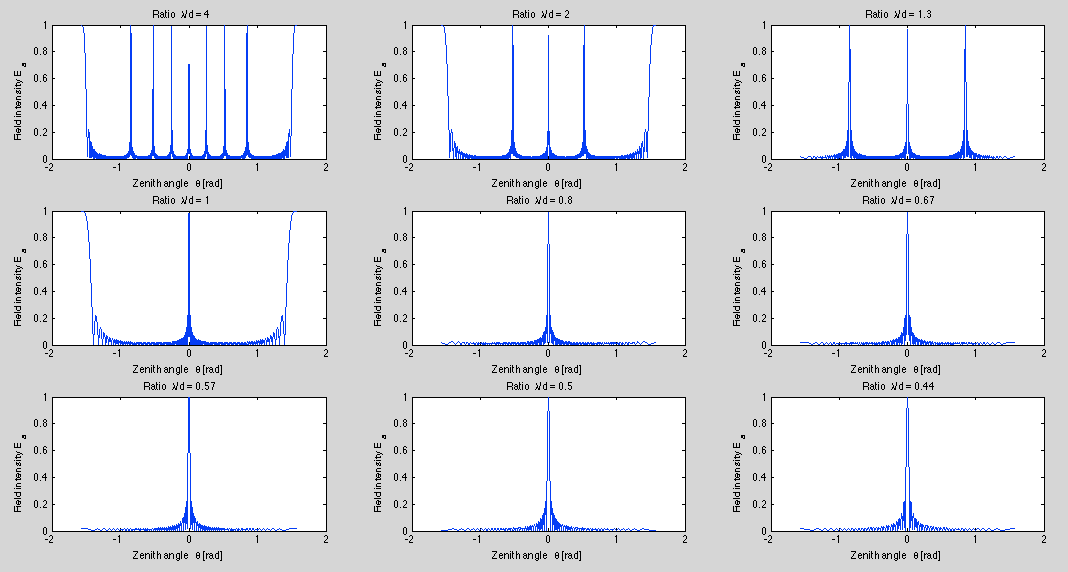
\includegraphics[width=\textwidth]{Figures/ratio.png}
\caption{Variation of the radiation pattern of a phased array antenna when the ratio between the wavelength and distance between individual elements varies.}
\label{fig:ratio}
\end{figure}

\begin{figure}[h!]
\centering
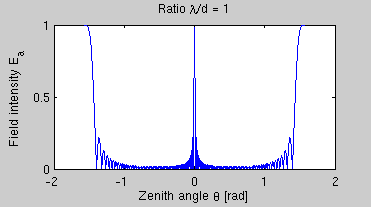
\includegraphics[width=\textwidth]{Figures/ratio_1.png}
\caption{Variation of the radiation pattern as zenith angle varies with $\lambda/d$ ratio as 1}
\label{fig:ratio_1}
\end{figure}

\begin{figure}[h!]
\centering
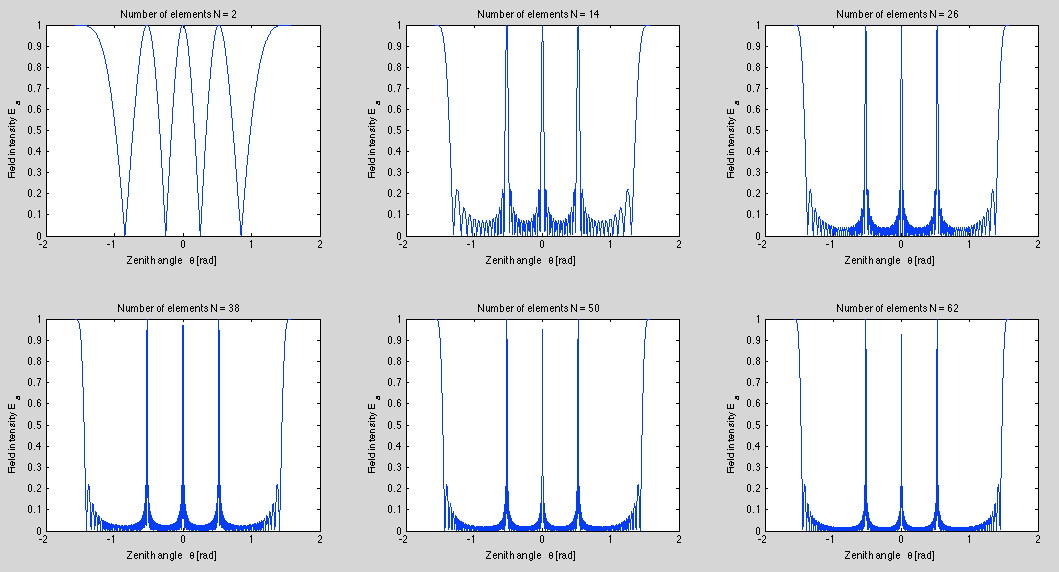
\includegraphics[width=\textwidth]{Figures/elements.png}
\caption{Variation of the radiation pattern of a phased array antenna when the number of elements of the antenna varies.}
\label{fig:elements}
\end{figure}

As shown in Figure \ref{fig:ratio_1}, when $\lambda = d$ there is one main lobe at $\theta = 0$ and lobes at $\theta =  \pm 90^{\circ}$.  In practice however the antenna elements are not isotropic and the radiation at $\pm 90^{\circ}$ is negligible. The width of the main lobe $sin^{-1}(\lambda/Nd)$. \cite{Rottger:2000ip}. The maxima other than the main lobe are called grating lobes. They are generally undesirable in that they can cause ambiguities by being mistaken for the response of a target in the main beam. Grating lobes can be avoided if the spacing \textit{d} between elements is equal to or less than $\lambda$.\cite{Skolnik:2001irs}. As can be seen from the Figure \ref{fig:ratio} grating lobes appear at angles $sin^{-1}(n\frac{\lambda}{d})$ \cite{Rottger:2000ip}\\

The Figure \ref{fig:elements} shows how the radiation pattern varies when the number of elements in the array is varied from $N = 2$ to $N = 62$. It can be clearly seen that the width of the lobes varies inversely with the number of elements in the array. As the number of elements in the array increases the width of the lobes decreases.\\

Therefore, in order to design a good MST radar the number of array elements should be sufficiently large and by theory the distance between these elements should be near to the wavelength being used. If N is large enough then the first side lobe is $13.2 dB$ lower than the main beam maximum value.\cite{Skolnik:2001irs}\\

The other way in which the side lobes can be suppressed further is by tapering of the antenna array which can be done either by changing the electrical weighting function $W_n$ (\textit{i.e.} by feeding outer elements with less power compared to the inner elements) or by unequal spacing of the array elements(\textit{i.e.} by using larger spacings for outer elements of the antenna array). The primary disadvantage of using these methods for side lobe suppression by tapering is the widening of the main lobe and lowering of the antenna gain \textit{G}.\cite{Rottger:2000ip}\\

Thus while designing a radar for atmospheric research a trade off has to be made between side lobe suppression and effective antenna aperture. A good effective aperture increases the sensitivity but does not suppress the side lobes. The suppression of side lobes by tapering methods attenuates the undesirable signals but decreases the gain of the antenna. So principally side lobe suppression is equivalent to a broadening of the antenna beam but this is considered to be a small problem compared to the difficult and lenghty procedures to remove the effects of side lobes from the main signal during data analysis procedures.\cite{Rottger:2000ip}\\


%----------------------------------------------------------------------------------------
%	SECTION 4. CONCLUSION
%----------------------------------------------------------------------------------------
%\newpage
\section{Conclusion}

This assignment has helped us get an idea of the design parameters of a phased array radar.
By varying the parameters that affect the design of a phased array antenna we observed how the radiation pattern varied. We learnt about the various techniques used for side lobe suppression in the radiation pattern. While doing this assignment we learnt about the trade off that has to be made between side lobe suppression and antenna gain in radars for MST weather applications. Finally we came to know about the parameters which are important while designing a practical phased array antenna.
%----------------------------------------------------------------------------------------
%	SECTION 5. REFERENCES
%----------------------------------------------------------------------------------------

\begin{thebibliography}{9}

\bibitem{Enmark:2012a3}
Enmark A.  (2012).
\newblock {\em Assignment 3. Optimization of phased array antenna radiation pattern and array configuration}.
\newblock Lule\aa \ University of Technology, Kiruna, Sweden.

\bibitem{Skolnik:2001irs}
Skolnik M. ~I.  (2001).
\newblock {\em Introduction to Radar Systems}.
\newblock The McGraw-Hill Companies, Inc., New York, United States.

\bibitem{Rottger:2000ip}
R\"ottger J.  (2000).
\newblock {\em The Instrumental Principles of MST Radars and Incoherent Scatter Radars and The Configuration of Radar System Hardware}.
\newblock Max Planck Institut F\"ur Aeronomie, Katlenburg-Lindau, Germany.

\bibitem{Wiki:2012pa}
Wikipedia.org. (2012).
\newblock {\em Phased array}.
\newblock {\url{http://en.wikipedia.org/wiki/Phased_array}}.

\end{thebibliography}


%----------------------------------------------------------------------------------------
%	SECTION 5. Appendix 1
%----------------------------------------------------------------------------------------
\newpage
\section{Appendix 1. Matlab code}
\lstinputlisting{assignment.m}

%----------------------------------------------------------------------------------------
%	SECTION 7. Confirmation
%----------------------------------------------------------------------------------------
\newpage
\section{Confirmation of Participation}

This is to confirm that the members of this team participated on the investigation of the required information to solve the assignment, generated their code to perform the calculation and discussed the results.\\
\vspace{2cm}
\newline
\line(1,0){200}\\
\authorivan\\
\vspace{2cm}
\newline
\line(1,0){200}\\
\authoranu\\


\end{document}